\section{Casi d'uso}

\subsection{Attori dei casi d'uso}

\subsubsection{Attori primari}
\begin{figure}[H]
		\centering
		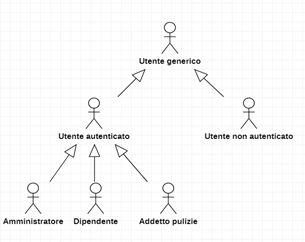
\includegraphics[width=10cm]{res/images/utentigenerali.png}
		\caption{Gerarchia degli attori principali}
		\label{fig:Gerarchia attori principali}
	\end{figure}

\textbf{Utente generico}\\
Si riferisce ad un utente generico che accede alla piattaforma.\\
\\
\textbf{Utente non autenticato}\\
Si riferisce ad un utente generico che non ha ancora effettuato l’autenticazione alla piattaforma.\\
\\
\textbf{Utente autenticato}\\
Si riferisce ad un utente generico che si è autenticato nel sistema con la procedura di login.\\
\\
\textbf{Amministartore}\\
Si riferisce ad un utente che si è autenticato nel sistema con il ruolo di amministratore.\\
\\
\textbf{Dipendente}\\
Si riferisce ad un utente che si è autenticato nel sistema con il ruolo di dipendente.\\
\\
\textbf{Addetto pulizie}\\
Si riferisce ad un utente che si è autenticato nel sistema con il ruolo di addetto alle pulizie.\\

\subsubsection{Attori secondari}
\textbf{Tag RFID}\\
Si riferisce ai tag presenti sulle postazioni. Ogni tag è assegnato ad una postazione e permette di identificarla digitalmente.\\
\\
\textbf{Ethereum}\\
Si riferisce al servizio che memorizza su blockchain gli eventi di occupazione e igienizzazione delle postazioni.\\

\subsection{Elenco dei casi d'uso}
In questa sezione sono riportati tutti i casi d'uso individuati, divisi per attore principale. Quando ritenuto utile essi sono accompagnati da un grafico.
\\
\subsubsection{ UC1 - Guida introduttiva}
\begin{itemize}
           	\item\textbf{Attori Primari:} utente generico;
           	\item\textbf{Descrizione:} L'utente riceve una guida riguardo il login e il funzionamento;
           	\item\textbf{Scenario principale:} l’utente accede alla pagina introduttiva e visualizza la guida;
           	\item\textbf{Precondizione:} il sistema è raggiungibile e funzionante, l’utente accede alla pagina iniziale del sito della piattaforma;
           	\item\textbf{Postcondizione:} il sistema fornisce all’utente, attraverso la lettura della guida, tutte le istruzioni necessarie ad effettuare il login;
\end{itemize}

\subsubsection{ UC2 - Login}
\begin{itemize}
           	\item\textbf{Attori Primari:} 
           	\item\textbf{Descrizione:} 
           	\item\textbf{Scenario principale:} 
           	\item\textbf{Precondizione:} 
           	\item\textbf{Postcondizione:}
\end{itemize}

\subsubsection{ UC3 - Logout}
\begin{itemize}
           	\item\textbf{Attori Primari:} 
           	\item\textbf{Descrizione:} 
           	\item\textbf{Scenario principale:} 
           	\item\textbf{Precondizione:} 
           	\item\textbf{Postcondizione:}
\end{itemize}

\subsubsection{ UC4 - Gestione impostazioni}
\begin{itemize}
           	\item\textbf{Attori Primari:} 
           	\item\textbf{Descrizione:} 
           	\item\textbf{Scenario principale:} 
           	\item\textbf{Precondizione:} 
           	\item\textbf{Postcondizione:}
\end{itemize}

\subsubsection{ UC5 -  Gestione stanze e postazioni}
\begin{itemize}
           	\item\textbf{Attori Primari:} 
           	\item\textbf{Descrizione:} 
           	\item\textbf{Scenario principale:} 
           	\item\textbf{Precondizione:} 
           	\item\textbf{Postcondizione:}
\end{itemize}

\subsubsection{ UC6 - Gestione credenziali dipendenti e addetti}
\begin{itemize}
           	\item\textbf{Attori Primari:} 
           	\item\textbf{Descrizione:} 
           	\item\textbf{Scenario principale:} 
           	\item\textbf{Precondizione:} 
           	\item\textbf{Postcondizione:}
\end{itemize}

\subsubsection{ UC7 - Esplorazione postazioni occupate da specifico utente}
\begin{itemize}
           	\item\textbf{Attori Primari:} 
           	\item\textbf{Descrizione:} 
           	\item\textbf{Scenario principale:} 
           	\item\textbf{Precondizione:} 
           	\item\textbf{Postcondizione:}
\end{itemize}

\subsubsection{ UC8 - Report sanificazioni postazione}
\begin{itemize}
           	\item\textbf{Attori Primari:} 
           	\item\textbf{Descrizione:} 
           	\item\textbf{Scenario principale:} 
           	\item\textbf{Precondizione:} 
           	\item\textbf{Postcondizione:}
\end{itemize}

\subsubsection{ UC9 - Visualizza stato postazione}
\begin{itemize}
           	\item\textbf{Attori Primari:} 
           	\item\textbf{Descrizione:} 
           	\item\textbf{Scenario principale:} 
           	\item\textbf{Precondizione:} 
           	\item\textbf{Postcondizione:}
\end{itemize}

\subsubsection{ UC10 - Segnalazione presenza}
\begin{itemize}
           	\item\textbf{Attori Primari:} 
           	\item\textbf{Descrizione:} 
           	\item\textbf{Scenario principale:} 
           	\item\textbf{Precondizione:} 
           	\item\textbf{Postcondizione:}
\end{itemize}

\subsubsection{ UC11 - Pulizia autonoma}
\begin{itemize}
           	\item\textbf{Attori Primari:} 
           	\item\textbf{Descrizione:} 
           	\item\textbf{Scenario principale:} 
           	\item\textbf{Precondizione:} 
           	\item\textbf{Postcondizione:}
\end{itemize}

\subsubsection{ UC12 - Prenotazione postazione}
\begin{itemize}
           	\item\textbf{Attori Primari:} 
           	\item\textbf{Descrizione:} 
           	\item\textbf{Scenario principale:} 
           	\item\textbf{Precondizione:} 
           	\item\textbf{Postcondizione:}
\end{itemize}

\subsubsection{ UC13 - Elenco stanze e postazioni da igienizzare}
\begin{figure}[H]
		\centering
		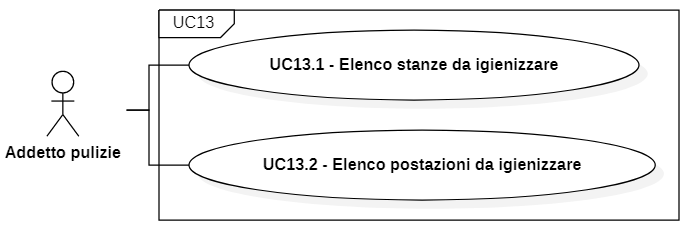
\includegraphics[width=15cm]{res/images/UC13.png}
		\caption{Elenco stanze e postazioni da igienizzare}
		\label{fig:Elenco stanze e postazioni da igienizzare}
	\end{figure}
\begin{itemize}
           	\item\textbf{Attori Primari:} addetto pulizie;
           	\item\textbf{Descrizione:} l'utente riceve un elenco delle postazioni[UC13.2] e delle stanze[UC13.1] che necessitano di igienizzazione;
           	\item\textbf{Scenario principale:} l'utente si trova all'interno del sistema e verifica tutte le postazioni che sono state utilizzate almeno da un dipendente che saranno quindi da igienizzare oppure può decidere di igienizzare l’intera stanza;;
           	\item\textbf{Precondizione:} l'utente va nella sezione dedicata nel sistema e deve premere un bottone;
           	\item\textbf{Postcondizione:} l'utente verifica quali postazioni sono state occupate da almeno un dipendente così da ottenere un elenco delle stanze e postazioni da igienizzare;
\end{itemize}

\subsubsection{UC13.1 - Elenco stanze da igienizzare}
\begin{itemize}
           	\item\textbf{Attori Primari:} addetto pulizie;
           	\item\textbf{Descrizione:} l'utente riceve un elenco delle stanza che necessitano di igienizzazione;
           	\item\textbf{Scenario principale:} l'utente si trova all'interno del sistema e verifica tutte le stanze che sono state utilizzate almeno da un dipendente 				che saranno quindi da igienizzare;
           	\item\textbf{Precondizione:} l'utente va nella sezione dedicata nel sistema e deve premere un bottone;
           	\item\textbf{Postcondizione:} l'utente verifica quali stanze sono state occupate da almeno un dipendente così da ottenere un elenco delle stanze da 				igienizzare;
\end{itemize}
\subsubsection{UC13.2 - Elenco postazioni da igienizzare}
\begin{itemize}
           	\item\textbf{Attori Primari:} addetto pulizie;
           	\item\textbf{Descrizione:} l'utente riceve un elenco delle postazioni che necessitano di igienizzazione;
           	\item\textbf{Scenario principale:} l'utente si trova all'interno del sistema e verifica tutte le postazioni che sono state utilizzate almeno da un dipendente 	che saranno quindi da igienizzare;
           	\item\textbf{Precondizione:} l'utente va nella sezione dedicata nel sistema e deve premere un bottone;
           	\item\textbf{Postcondizione:} l'utente verifica quali postazioni sono state occupate da almeno un dipendente così da ottenere un elenco delle postazioni da igienizzare;
\end{itemize}

\subsubsection{ UC14 - Marcatura stanza e postazione come igienizzata}
\begin{figure}[H]
		\centering
		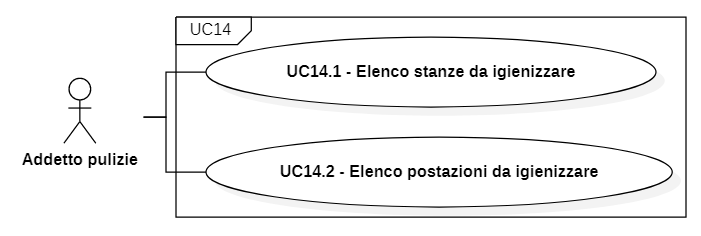
\includegraphics[width=18cm]{res/images/UC14.png}
		\caption{Marcatura stanza e postazione come igienizzata}
		\label{fig:Marcatura stanza e postazione come igienizzata}
	\end{figure}
\begin{itemize}
           	\item\textbf{Attori Primari:} Addetto pulizie;
		\item\textbf{Attori Secondario:} Ethereum;
           	\item\textbf{Descrizione:} dopo l'igienizzazione l'utente marca le stanze o le postazioni che ha pulito come igienizzate;
           	\item\textbf{Scenario principale:} l'utente igienizza la stanza[UC14.1] o la postazione[UC14.2] e in seguito accede al sistema e la marca come igienizzata attraverso l'utilizzo di ethereum;
           	\item\textbf{Precondizione:} l'utente ottiene l'elenco delle stanze e delle postazioni da igienizzare;
           	\item\textbf{Postcondizione:} l'utente, dopo l'igienizzazione, marca le stanze e le postazioni come igienizzate;
\end{itemize}
\subsubsection{UC14.1 - Marcatura stanza come igienizzata}
\begin{itemize}
           	\item\textbf{Attori Primari:} Addetto pulizie;
		\item\textbf{Attori Secondario:} Ethereum;
           	\item\textbf{Descrizione:} dopo l'igienizzazione l'utente marca la stanza come igienizzata;
           	\item\textbf{Scenario principale:} l'utente igienizza la stanza e in seguito accede al sistema e la marca come igienizzata attraverso l'utilizzo di ethereum;
           	\item\textbf{Precondizione:} l'utente ottiene l'elenco delle stanze da igienizzare;
           	\item\textbf{Postcondizione:} l'utente, dopo l'igienizzazione, marca le stanze come igienizzate;
\end{itemize}
\subsubsection{UC14.2 - Marcatura postazione come igienizzata}
\begin{itemize}
           	\item\textbf{Attori Primari:} Addetto pulizie;
		\item\textbf{Attori Secondario:} Ethereum;
           	\item\textbf{Descrizione:} dopo l'igienizzazione l'utente marca la postazione come igienizzata;
           	\item\textbf{Scenario principale:} l'utente igienizza la postazione e in seguito accede al sistema e la marca come igienizzata attraverso l'utilizzo di ethereum;
           	\item\textbf{Precondizione:} l'utente ottiene l'elenco delle postazioni da igienizzare;
           	\item\textbf{Postcondizione:} l'utente, dopo l'igienizzazione, marca le postazioni come igienizzate;
\end{itemize}
